\documentclass[conference]{IEEEtran}
\usepackage{times}

% numbers option provides compact numerical references in the text. 
\usepackage[numbers]{natbib}
\usepackage{multicol}
\usepackage[bookmarks=true]{hyperref}
\usepackage{graphics} % for pdf, bitmapped graphics files
\usepackage{graphicx}
\usepackage{amsmath,amssymb,latexsym,float,epsfig,subfigure}
\usepackage{amsmath} % assumes amsmath package installed
\usepackage{amssymb}  % assumes amsmath package installed
\usepackage{lipsum}
\usepackage[export]{adjustbox}
\usepackage[normalem]{ulem} % underline
\usepackage{wrapfig}
\usepackage{multirow}
\usepackage{balance}
\usepackage{color}
\usepackage{url}
\usepackage{booktabs}
\newcommand{\argmax}{\arg\!\max}
\newcommand{\norm}[1]{\left\lVert#1\right\rVert}
\pdfinfo{
   /Author (Deepak Gopinath, Brenna D. Argall)
   /Title  (Mode Switch Assistance to Human Intent Disambiguation)
   /CreationDate (January 31 2017)
   /Subject (Robots)
   /Keywords (Robots)
}

\begin{document}

% paper title
\title{Mode Switch Assistance to\\Maximize Human Intent Disambiguation}
\author{Author Names Omitted for Anonymous Review. Paper-ID [\textbf{163}]}
% You will get a Paper-ID when submitting a pdf file to the conference system
%\author{Deepak Gopinath and Brenna D. Argall}

%\author{\authorblockN{Deepak Gopinath}
%\authorblockA{Department of Mechanical\\Engineering,
%Northwestern University\\
%Evanston, Illinois 30332\\
%Email: deepakedakkattilgopinath2015\\@u.northwestern.edu}
%\and
%\authorblockN{Brenna D. Argall}
%\authorblockA{Department of Mechanical\\Engineering,
%		Northwestern University\\
%		Evanston, Illinois 30332\\
%		Email: brenna.argall@northwestern.edu}
%	}

%\author{Deepak Gopinath$^{1}$ and Brenna D. Argall$^{2}$
%	\thanks{Manuscript received: March, 1, 2016; Revised June,
%		7, 2016; Accepted June, 29, 2016.}
%}
% avoiding spaces at the end of the author lines is not a problem with
% conference papers because we don't use \thanks or \IEEEmembership


% for over three affiliations, or if they all won't fit within the width
% of the page, use this alternative format:
% 
%\author{\authorblockN{Deepak Gopinath\authorrefmark{1}\authorrefmark{2},
%Brenna D. Argall\authorrefmark{1}\authorrefmark{2}\authorrefmark{3}\authorrefmark{4}
%}
%\authorblockA{
%	\authorrefmark{1}Department of Mechanical Engineering, Northwestern University, Evanston, IL}
%
%\authorblockA{\authorrefmark{2}Rehabilitation Institute of Chicago, Chicago, IL}
%
%\authorblockA{\authorrefmark{3}Department of Physical Medicine and Rehabilitation, Northwestern University, Chicago, IL}
%
%\authorblockA{\authorrefmark{4}Department of Electrical Engineering and Computer Science, Northwestern University, Evanston, IL}
%
%\authorblockA{{\tt\small deepakedakkattilgopinath2015@u.northwestern.edu}}
%\authorblockA{{\tt\small brenna.argall@northwestern.edu}}
%}


\maketitle

\begin{abstract}
%In this paper, we propose a mathematical framework which formalizes user-driven customization of shared autonomy in assistive robotics as a nonlinear optimization problem. 
%Our insight is to allow the \textit{end-user}, rather than relying on standard optimization techniques, to perform the optimization procedure, thereby allowing us to leave the exact nature of the cost function indeterminate.
%We ground our formalism with an interactive
%optimization procedure that customizes
%control sharing using an assistive robotic arm. We also present
%a pilot study that explores interactive optimization with
%end-users.
%This study was performed with 17 subjects (4 with spinal cord injury, 13 without injury). Results
%show all subjects were able to converge to an assistance paradigm, suggesting the existence of optimal solutions. Notably, the amount of assistance was not always
%optimized for task performance. Instead, some subjects
%favored retaining more control during the execution over better task
%performance.
%The study supports the case for user-driven customization and provides
%guidance for its continued development and study.

In this paper, we develop an algorithm for goal disambiguation with a shared-control assistive robotic arm. Assistive systems are often required to infer human intent and this usually becomes a bottleneck for providing assistance quickly and accurately. We introduce the notion of \textit{inverse legibility} in which the human-generated actions are legible enough for the \textit{robot} to infer the human intent confidently and accurately. The proposed disambiguation paradigm seeks to elicit legible control commands from the human by selecting control modes that \textit{maximally disambiguate} between the various goals in the scene. We present simulation results which look into the robustness of our algorithm and the impact of the choice of confidence functions on the performance of the system. Our simulation results suggest that the disambiguating control mode computed by our algorithm produces more intuitive results when the confidence function is able to capture the ``directedness'' towards a goal. We also present a pilot study that explores the efficacy of the algorithm on real hardware. Preliminary results indicate that the assistance paradigm proposed was successful in decreasing task effort (number of mode switches) across interfaces and tasks. 
\end{abstract}

\IEEEpeerreviewmaketitle

\section{Introduction}

Assistive and rehabilitation devices such as powered wheelchairs, robotic arms and myoelectric prostheses play an important role in the lives of people with motor impairments. These devices help to increase their ability to perform activities of daily lives and reduce their dependence on caretakers, and are crucial to revolutionizing the way they interact with society. As the field of assistive robotics progresses rapidly, the devices themselves become more capable and dextrous---and as a result also more complex, high dimensional and harder to control. 

The common paradigm for control of such high-dimensional devices has the human directly control the motion via a control interface. The confounding factor is that the more severe a person's motor impairment, the more limited are the control interfaces available to them to operate. These interfaces (for example,  a switch-based head array and Sip-N-Puff) are lower in dimensionality and bandwidth, and usually require more mode switches for successful task completion. Thus, a greater need for sophisticated assistive devices is paired with a diminishing ability to control their additional complexity. 

Due to the dimensionality mismatch between the control interface and the robotic device, control interfaces operate in \textit{modes} which correspond to different partitions of the control space. Typically, the more limited the control interface is, the greater number of modes there are. In order to have full control of the robot the user will have to switch between the difference partitions of the control space and this is known as \textit{mode switching}. 

It has been established that mode switching is expensive and as a result task performance is degraded. Furthermore, it adds to the cognitive and physical burden as each of these mode switches requires the user to shift their attention from the task to performing the mode switch. The introduction of \textit{shared autonomy} to these systems helps to alleviate and address some of these issues by letting the system take responsibility to some extent, thereby reducing the human effort in achieving a goal. 

For any assistive autonomy, the system typically needs an idea of what it is the human is trying to do---either by explicit indication from the user of the task or goal~\cite{choi2008laser}, or by inferring the human's intent from their control signals and/or sensor data. The question of intent inference is key. In this paper, we develop an assistance paradigm that helps with intent inference, by selecting the control mode in which robot motion will \textit{maximally disambiguate} human intent. In general, the faster the autonomy is able to disambiguate intent, the earlier the robot is able to provide autonomy assistance---leading ideally to fewer mode switches and less burdensome executions. 

%Shared autonomy paradigms in assistive robotics can be broadly classified into two categories: \textit{hierarchical} and \textit{blending}. \textit{Hierarchical} assistance paradigm is one in which the user takes care of the higher level aspects of the task and the robot is responsible for the low level control and planning needed for successful task execution. An example of a \textit{hierarchical} assistance system is a smart wheelchair system in which the user can specify the goal using a touchpad interface and the robot uses local and global planners to successfully accomplish the navigation task. On the other hand, in a \textit{blending}--based assistance paradigm, the robot and the human work in the same control space (for example, velocity blending in Cartesian space) and usually the final control command issued to the robot is a blended sum of an autonomous robot policy and the control command issued by the human.
\begin{figure}[t]
	\centering
	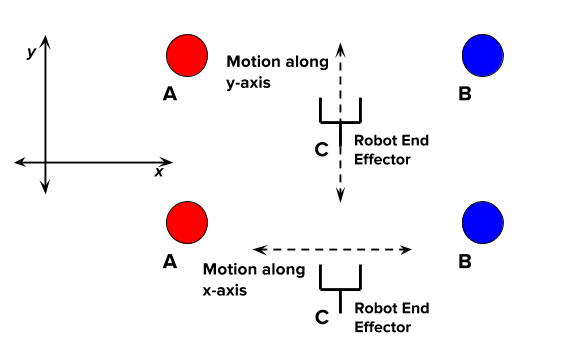
\includegraphics[width = 1.0\hsize]{./figures/DE.png}
	\vspace{-0.7cm}
	\caption{Illustration of goal disambiguation along various control dimensions. A and B indicate two point goal locations. The robot end effector is at location C. Any motion of the end effector along the y-axis will not help the system to disambiguate between the two goals; that is, the motion is not legible. However, motion along the x-axis allows the goal to be inferred immediately based on the direction in which the robot moves. }
	\label{DE}
\end{figure}

%In this paper, we develop a mode switching assistance paradigm that augments an underlying blending--based shared control system for an assistive robotic arm.
 In many shared-control systems, the assistance provided by the robot is regulated by the robot's ability to estimate user intent confidently and accurately, and it is very unlikely that the robot will be able to determine this with a 100\% accuracy.  Therefore in the literature to date, the factor dictating how much control lies with the robot versus with the human is usually a function of a confidence metric. This confidence metric is the system's confidence in its own estimate of human intent and is usually a function of the human control command, the autonomous policy, robot pose, goal locations, \textit{et cetera}. This implies that human control actions can potentially have a direct impact on the confidence measure. 

The concept of \textit{legibility} is typically used in the domain of Human-Robot Interaction (HRI) as applied to robot motion. A \textit{legible} motion in this context is one which will help the observer (usually the human) decipher the intent behind the robot's action more \textit{quickly} and \textit{confidently}. However, it can be the case that certain actions \textit{by} the human might carry more information than others and better express the human's intent, which can then help the robot to draw useful and correct inferences more easily. Therefore, in this paper we propose a paradigm of \textit{inverse legibility} in which the roles are switched and the human-generated actions \textit{help the robot} to infer human intent confidently and accurately. 
%\textbf{[Can there be a concept of bilateral legibility? The human knows the goal. And therefore has a model for what a predictable motion is. If the robot indeed performs that predictable motion, there is an agreement between the expectation and what really happened. That is, the robot motion becomes legible.]}

Consider the example illustrated in Figure~\ref{DE}. In this example, a human control command issued along the $x$ dimension is more \textit{intent expressive} and helps the robot to provide the right kind of assistance quickly and confidently. With the disambiguation assistance scheme developed in this work, we hope to elicit more legible human control commands by placing the user control in those modes with \textit{maximum disambiguation} between the various goals in the scene. 

%The commonplace notion in human-robot interaction and especially in assistive robotics is that ``help'' is provided solely by the robot. In addition to eliciting more legible motion from the human, we also seek to explore and exploit the underlying synergies in human robot interaction to facilitate more seamless and efficient task execution. The idea of \textit{``people helping robots helping people''} is key here and by requiring the human to operate in a mode that will potentially help the robot in deciphering the intent the human, in some sense, helps the robot to perform more effectively.
%It is possible that in some cases such a mode might not be the most ideal mode \textit{for} the human to operate in due to personal preferences. However, if the human agrees to compromise a little bit and provides ``hints" and ``nudges" the robot in the right direction, the overall performance gain will likely outweigh the slight sub-optimality due to the ``wrong'' mode. 

In Section \ref{RW} we present an overview of relevant research in the area of shared control in assistance systems focusing on mode switching, legibility and synergies in HRI. Section \ref{ALGO} describes the mathematical formalism for the algorithm and the metric used for goal disambiguation. The empirical methods are outlined in Section~\ref{EV} followed by simulation results in Section~\ref{SIMRESULTS}. The pilot study methods, metrics and results are discussed in Section \ref{EXP}, followed by conclusions in Section \ref{DC}.

\section{RELATED WORKS}\label{RW} 

Shared-control assistance paradigms help to offload cognitive and physical burden~\cite{volosyak2005rehabilitation} without requiring the user to relinquish complete control, and are usually preferred over fully autonomous assistive robotic systems for reasons of both robustness and user satisfaction. One possible way to control high-dimensional assistive devices such as robotic arms is to partition the control space (often 6D for a robotic arm) into subsets called \textit{modes} and have the user control one mode at a time using control interfaces such as joysticks, head arrays and sip-and-puffs~\cite{tsui2008development, nuttin2002selection}. This is known as \textit{modal control}.

Herlant \textit{et al.}~\cite{herlant2016assistive} assesses the difficulties faced by users when they operate assistive devices using \textit{modal control}. In their work they report that a significant number of users found \textit{mode switching} to be slow and burdensome. The cognitive burden of shifting focus (\textit{task switching})  from the task at hand to mode switches can result in a significant decrease in task performance regardless of the control modality~\cite{monsell2003task}. 

 A time-optimal mode switch assistance paradigm evaluated on a simulated 2D robot provides insight into the fact that even a simple time-optimal automatic mode switching system can significantly improve user satisfaction while maintaining the quality task performance~\cite{herlant2016assistive}.  Another study~\cite{gopinath2017human} found that it is not always the case that users are trying to optimize for time or effort during task execution. However, our present system therefore does not make \textit{a priori} assumptions regarding the optimizing principles at work when a user operates a robot.

The legibility and predictability of robot motion \textit{to the human} have been thoroughly investigated~\cite{dragan2013legibility}, and different methods for generating legible robot motion have been proposed by Holladay \textit{et al}~\cite{holladay2014legible}. We apply similar concepts of legibility however to the \textit{human control} commands, such that the intent expressed in the human command is clear \textit{to the robot}. Our assistance scheme is intended to bring out a more legible intent-expressive control command from the human, so that the autonomy is able to infer the correct goal more confidently. 
%In most cases the human knows beforehand what goal he/she is going for and therefore the motion generated by the human is usually \textit{predictable}.
As long as the confidence measure used to disambiguate between candidate goals captures the predictable aspect of human-generated robot motion, our proposed disambiguation assistance will place user control in that mode which can provide maximal goal disambiguation and improved legibility.

Also related to our work is the idea of mutual cooperation between humans and robots, and the underlying synergies that are crucial for successful human-robot interaction. The commonplace notion in human-robot interaction, and especially in assistive robotics, is that ``help'' is provided solely by the robot. In addition to eliciting more legible motion from the human, we also seek to exploit the underlying synergies in human-robot interaction to faciliate more seamless and efficient task execution. From the robot's perspective the key concept behind our algorithm is the idea of \textit{``Help Me, Help You''}---that is, if the human can ``help'' the robot by providing more legible control commands, then the robot in turn can assist the human even more effectively. This concept has been explored by Goodfellow \textit{et. al}~\cite{goodfellow2010help} for developing user interfaces that overcome the communication bottleneck that exists between robots and people by accounting for the constrained capabilities of a robot. Sorokin \textit{et al.}~\cite{sorokin2010people} proposes a framework for \textit{``people helping robots helping people''} in which humans provide semantic information and judgments about the environment to the robot which then utilizes them to improves its own capabilities.  Rosenthal \textit{et al.}~\cite{rosenthal2010effective} proposes a \textit{symbiotic} human robot interaction scheme which aims to overcome perceptual and cognitive limitations that robots might encounter while still allowing the robots to help humans as well. 


%2-4 works which investigates what legibility means, proposes ways to generate legible robot motion. In all these works, the goal is to make the motion more legible for the human. In our system, we want the human to move the robot in a way that the intent is more legible FOR the system. That is the roles are reversed. Since the human knows beforehand what goal he/she is going after the motion generated by the human is usually predictable. As long as the confidence measure is able to capitalize on this predictability, the system can force the human to generate legible motions by requiring them to operate in those modes which can provide maximal confidence disambiguation. The notion of a confidence mediated blending paradigm is formalized in other Dragan paper. 
%
%Discuss works which formalizes legibility. Talk about how in the present work we are flipping roles and concerned more about the legibility of human's actions (which causes robot motion). Dragan et al. formalizes and investigates legibility and predictability of robot motion. Their paper's concern was primarily to make a robot's motion more legible for the human who will the observer. In the present work, we use the principle of legibility, except that the robot and the human switch roles. The human controls the robot motion via a control interface and robot is the ``observer'' and the system seeks to elicit to legible indicators \textit{from} the human in order to provide more effective assistance.

%Discuss works which emphasize two way interaction for more gain. Look into this a little more closely. Synergy related work. 
\begin{figure}
%	\centering
	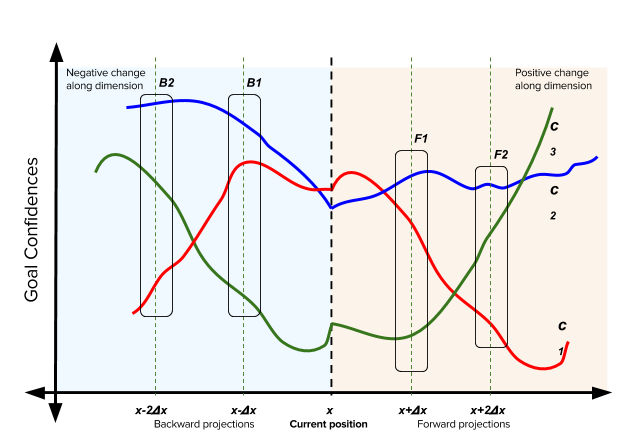
\includegraphics[width = 1\hsize, height = 0.26\vsize]{./figures/DisambMetric.png}
	\vspace{-0.4cm}
	\caption{Illustration of change in confidence with movement along a single control dimension. The region accessible from position \textit{x} due to positive and negative motion is shaded beige and light blue respectively. Note the discontinuity in the confidences at the current position.}
	\label{DM_FIG}
\end{figure}
\section{ALGORITHM DESIGN} \label{ALGO}
This section describes the algorithm that is used to compute the control mode with maximum goal disambiguation, thereby eliciting the most legible control command from the human. Section~\ref{NOT} outlines the mathematical notation used in the paper and Section~\ref{CF} discusses various confidence functions. Section~\ref{DM} describes the different considerations that inform the confidence disambiguation metric. The details of the underlying shared control system is also described briefly in this Section~\ref{BP}.

\subsection{Notation}\label{NOT}

%Let $g_i \in \mathcal{G} \;\; \forall \;\;i \in [1,2,\dots,n_g]$, denote the $n_g$ number of possible goals in the scene and $c_i \in \mathcal{C} \;\; \forall \;\;i \in [1,2,\dots,n_g]$ denote the confidence that the system has in each one of the $n_g$ goals.

Let $\mathcal{G}$ be the set of all candidate goals in the scene with $n_g = \vert\mathcal{G}\vert$ and let $g^{i}$ refer to the $i^{th}$ goal where $i \in [1,2,\dots,n_g]$. The set of goals results in an associated set of confidences denoted as $\mathcal{C}$, where $c^{i}$ refers to the individual confidence associated with goal $g^{i}$. Let $\mathcal{K}$ be the control space in which the robot operates and $k^{i}$ refer to an individual control dimension where $i \in [1,2,\dots,n_k]$.  The cardinality of $\mathcal{K}$ depends on the robotic platform; for example, for a smart wheelchair $n_k = 2$ whereas for a 6 DOF robotic arm $n_k = 6$.
%Let $\mathcal{G}$ be the set of all candidate goals in the scene with $\vert\mathcal{G}\vert = n_g$, resulting in an associated distribution of confidences $c_g \in \mathcal{C} \;\;( \forall \; g \in \mathcal{G})$  over candidate goals. Let $\mathcal{K}$ be the control space in which the robot operates with $\vert\mathcal{K}\vert = n_k$.

For control purposes, the set $\mathcal{K}$ is partitioned into subsets known as \textit{modes}. Let $\mathcal{M}$ refer to the set of all modes that the control space $\mathcal{K}$ is partitioned into with $n_{m} = \vert\mathcal{M}\vert$. The number of modes ($n_{m}$) is specific to the control interface and mapping to $\mathcal{K}$. Furthermore, let $m^{i}$ refer to the $i^{th}$ mode where $i \in [1,2,\dots,n_{m}]$.

Another quantity of interest is the gradient of individual goal confidences along the different control dimensions. More specifically, $\frac{\partial c}{\partial k}$ captures the rate of change of the confidence $c$ along control dimension $k$. Furthermore, since the confidence function, in general, can assume drastically different values upon moving in positive and negative directions along a  given control dimension, the positive and negative gradients are explicitly denoted as $\frac{\partial c}{\partial k}^{+}$ and $\frac{\partial c}{\partial k}^{-}$ respectively. The formalism developed in Section~\ref{DM} is agnostic to a particular form of confidence function. Additionally, an analytical closed-form expression for the gradient might not always be available as the confidence functions need not be continuous and differentiable. Even when available, due to the complexity of the confidence measure such an expression might be expensive to compute. Therefore in our work, the gradient is numerically approximated.
%Lastly, we define a \textit{disambiguation} metric $D_{k_j}\in \mathbb{R}\; \forall \;k_j \in \mathcal{K}$ and is a function of the individual goal confidences $c_i$ and $\frac{\partial c_i}{\partial k_j}$\footnote{For the rest of the paper $\frac{\partial c_i}{\partial k_j}$ will be denoted as $ \dot{c}_{ij}$}. 

We define a \textit{disambiguation} metric, $D_{k}\in \mathbb{R}$ for each control dimension $k \in \mathcal{K}$, which is a function of $c$ and $\frac{\partial c}{\partial k}$. Analogous to the gradients, we explicitly define disambiguation metrics for both positive and negative motion directions as $D_{k}^{+}$ and $D_{k}^{-}$ respectively.

We further define a disambiguation metric $D_m \in \mathbb{R}$ for each control mode $m \in \mathcal{M}$.
The disambiguation metric $D_m$ is a measure of how legible the user commands would be if the user were to control the robot in mode $m$. The higher the value, the easier it will be for the system to infer the human's intent. 
\subsection{Confidence function}\label{CF}
The choice of confidence function is entirely up to the system designer and numerous options exist. An example of a simple distance-based confidence function is
\begin{equation*}\label{EQ1}
c(\boldsymbol{x}, \boldsymbol{x_g}) = \max(0, 1 - \frac{\norm{\boldsymbol{x} - \boldsymbol{x}_{g}}}{D})
\end{equation*}
where $\boldsymbol{x}$ is the current position of the robot, $\boldsymbol{x}_{g}$ is the location of goal $g$, $D$ is the radius of a sphere beyond which the confidence is always $0$ and $\norm{\cdot}$ is the Euclidean norm. We refer to this confidence function as \textbf{C1}. However, this confidence measure ignores all cues regarding human intent present in the control command itself. Therefore a better choice of confidence function should try to capture the ``directedness'' of the human control command towards a goal. One option is
\begin{equation*}\label{EQ2}
c({\boldsymbol{x},\boldsymbol{x_g}, \boldsymbol{u}_{h}}) = \boldsymbol{u}_h\cdot(\boldsymbol{x}_{g} - \boldsymbol{x})
\end{equation*}
where $\boldsymbol{u}_h$ is the human control command. We refer to this confidence function as \textbf{C2}. \textbf{C1} and \textbf{C2} can be combined into a single function to capture both ``proximity'' to and ``directedness'' towards a goal.
%\begin{equation}\label{EQ3}
%c^i({\boldsymbol{x}, \boldsymbol{u}_{h}}) = \boldsymbol{u}_h\cdot(\boldsymbol{x}_{g^i} - \boldsymbol{x}) + \max(0, 1 - \frac{\norm{\boldsymbol{x} - \boldsymbol{x}_{g^i}}}{D})
%\end{equation}

Furthermore, the control signal from the robot autonomy is generated by a function $f_{r}(\cdot) \in \mathcal{F}_{r}$, 
\begin{equation*}
\boldsymbol{u}_r \leftarrow f_{r}(\boldsymbol{x})
\end{equation*}
where $\mathcal{F}_{r}$ is the set of all control behaviors corresponding to different tasks. The algorithm proposed in this paper requires that the confidence measures varies as a function of $\boldsymbol{x}$, so that $\frac{\partial c}{\partial k}$ is well-defined and exists. The specific form of the confidence function and the autonomous robot policy generator will be discussed in Section~\ref{BP}.
\subsection{Disambiguation metric}\label{DM}
Let the component of $\boldsymbol{x}$ along control dimension $k$ be denoted as $x$. 
Figure~\ref{DM_FIG} is an illustrative example which shows how goal confidences can vary as a function of position along a control dimension. 

The disambiguation metric $D_{k}$ encodes different aspects of how the goal confidences change upon moving (either in the positive or negative direction) along control dimension $k$. A proper design of $D_{k}$ should take into account both immediate as well as long term benefits of moving in $k$ and combine them into one metric. We identify four important considerations to  inform the design of $D_{k}$.

\subsubsection{Separation in confidences}
A good measure for evaluating the confidence disambiguation potential of a control dimension is to compute the \textit{separation}, $\Lambda_{k}$, in goal confidences. At any point in space this can be computed as the \textit{sum of pairwise distances} between the $n_g$ confidences. Since we are interested in the separation after a small change in position (due to user-initiated robot motion), we can sample the confidence function at $x\pm\Delta x$ and use the sampled values to compute $\Lambda_{k}$, where $\Delta x$ is a small change along the control dimension. Thus,
\begin{equation*}
\Lambda_{k} = \sum_{p=1}^{n_g}\sum_{q=p}^{n_g}\lvert c^{p}_{\delta_x} - c^{q}_{\delta_x}\rvert
\end{equation*}
where $\delta_x$ indicates $x+\Delta x$ or $x-\Delta x$ depending on the direction of perturbation and $\lvert\cdot\rvert$ denotes the absolute value. 
\subsubsection{Max of confidences}
The maximum of the goal confidences is a good measure of the system's overall certainty in accurately estimating human intent. A higher maximum implies that the robot has an even better idea of and is fairly sure of what the human is trying to do. The max ($\Gamma_{k}$) is computed as
\begin{equation*}
%M^{\pm}_{k^j} = \sum_{p = 1}^{n_g}c^{p}_{x_{j}^{\delta\pm}}.
\Gamma_{k} =\max\limits_{1 \leq i \leq n_g}c^{i}_{\delta_x}
\end{equation*}
\subsubsection{Difference between largest confidences}
%For the blending paradigm, the current goal ($\boldsymbol{g}^{*}$) is the one with the highest confidence value. That is, 
%\begin{equation*}
%\boldsymbol{g}^{*} = g^{\argmax_i c^i}
%\end{equation*}
%
%Therefore, it is crucial that the difference between the largest and the second largest confidences in $\mathcal{C}$ is significant so that the computation of $\argmax_i c^i$ is likely to generate the current predicted goal. Any ambiguity will likely result in a less accurate prediction of $\boldsymbol{g}^*$. 
Since it is possible to have multiple\footnote{Note that confidences are not normalized, since we do care about more than just their relative magnitudes as in bullet 2.} highly confident goals, accurate disambiguation also benefits from a large separation between the first and second most confident goals. 
This difference is denoted by $\Delta_{k}$ and is computed as
\begin{equation*}
\Delta_{k} = \max(\mathcal{C}) - \max(\mathcal{C} \setminus {\max(\mathcal{C})})
\end{equation*}
\subsubsection{Gradients}
The propensity for change and information gain upon the continuation of motion along control dimension $k$ is encoded in the gradients $\frac{\partial c}{\partial k}\; \forall\; c\in \mathcal{C}$. The greater the difference between the gradients of individual confidences $c$, the greater will they deviate from each other.  Instead of using closed-form analytical gradients, we approximate the gradients using forward and backward differences. Therefore, 
\begin{equation*}
\frac{\partial c}{\partial k} \approx c_{\delta_x} - c_{x} 
\end{equation*}
where $c_x$ denotes the confidence at location $x$.
In order to quantify the ``spread'' of gradients we define a quantity $\Upsilon_{k}$ which is computed as 
\begin{equation*}
\Upsilon_{k} = \sum_{p=1}^{n_g}\sum_{q=p}^{n_g}\Big \lvert\frac{\partial c^p}{\partial k} - \frac{\partial c^q}{\partial k}\Big \rvert
\end{equation*}

\subsubsection*{Putting it all together}
$\Lambda_{k}$, $\Gamma_{k}$, $\Delta_{k}$ and $\Upsilon_{k}$ are then combined to compute $D_{k}$ as 
\begin{equation}\label{DK}
D_{k} = \underbrace{\boldsymbol{w}\cdot(\Lambda_{k}\cdot \Gamma_{k}\cdot \Delta_{k})}_{\text{long term}} + \underbrace{(1 - \boldsymbol{w})\cdot \Upsilon_{k}}_{\text{short term}}
\end{equation}
where $\boldsymbol{w}$ controls the relative contribution of immediate and the long term benefit. Equation~\ref{DK} actually is computed twice, once in each of the positive ($\delta_x = x + \Delta x$) and negative directions ($\delta_x = x - \Delta x$), and the results are then summed. 
Once the disambiguation metric $D_k$ for each control dimension $k$ is computed, the disambiguation metric $D_m$ for control mode m is calculated as 
\begin{equation*}
D_m = \sum_{j} D_{k} \; \forall \; k \in m
\end{equation*}
The control dimension with highest disambiguation capability $\boldsymbol{k}^*$ is given by
\begin{equation*}
\boldsymbol{k}^* = \argmax_k D_{k}
\end{equation*}
 and the mode with highest disambiguation capability $\boldsymbol{m}^{*}$ is given by
\begin{equation*}
\boldsymbol{m}^* = \argmax_m D_m
\end{equation*}
Disambiguation mode $\boldsymbol{m}^{*}$ is the mode that the algorithm chooses \textit{for} the human to better their intent. Any subsequent control command issued by the user in $\boldsymbol{m}^*$ is likely to be more legible due to maximal goal confidence disambiguation.

\subsection{Blending paradigm}\label{BP}
\begin{wrapfigure}[9]{R}{0.2\textwidth}
	\begin{center}
		\vspace{-0.9cm}
		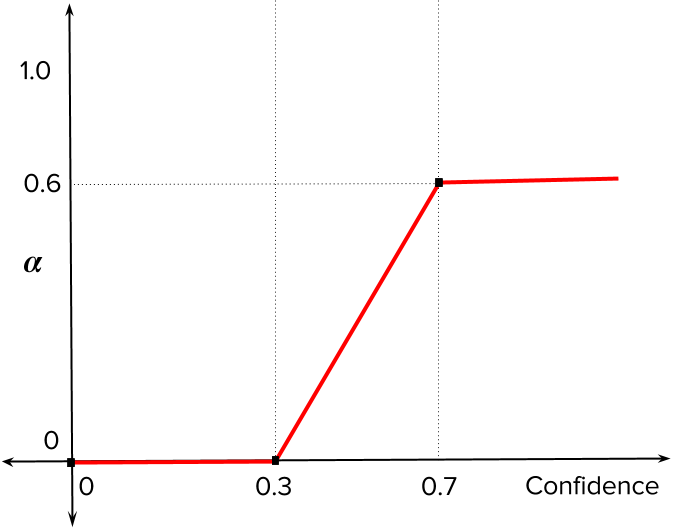
\includegraphics[width=0.2\textwidth]{./figures/ArbFunc.png}
	\end{center}
		\vspace{-.45cm}
	\caption{A prototypical arbitration function.}
	\label{ALPHA}
\end{wrapfigure}
\begin{figure*}[ht]
	\centering
	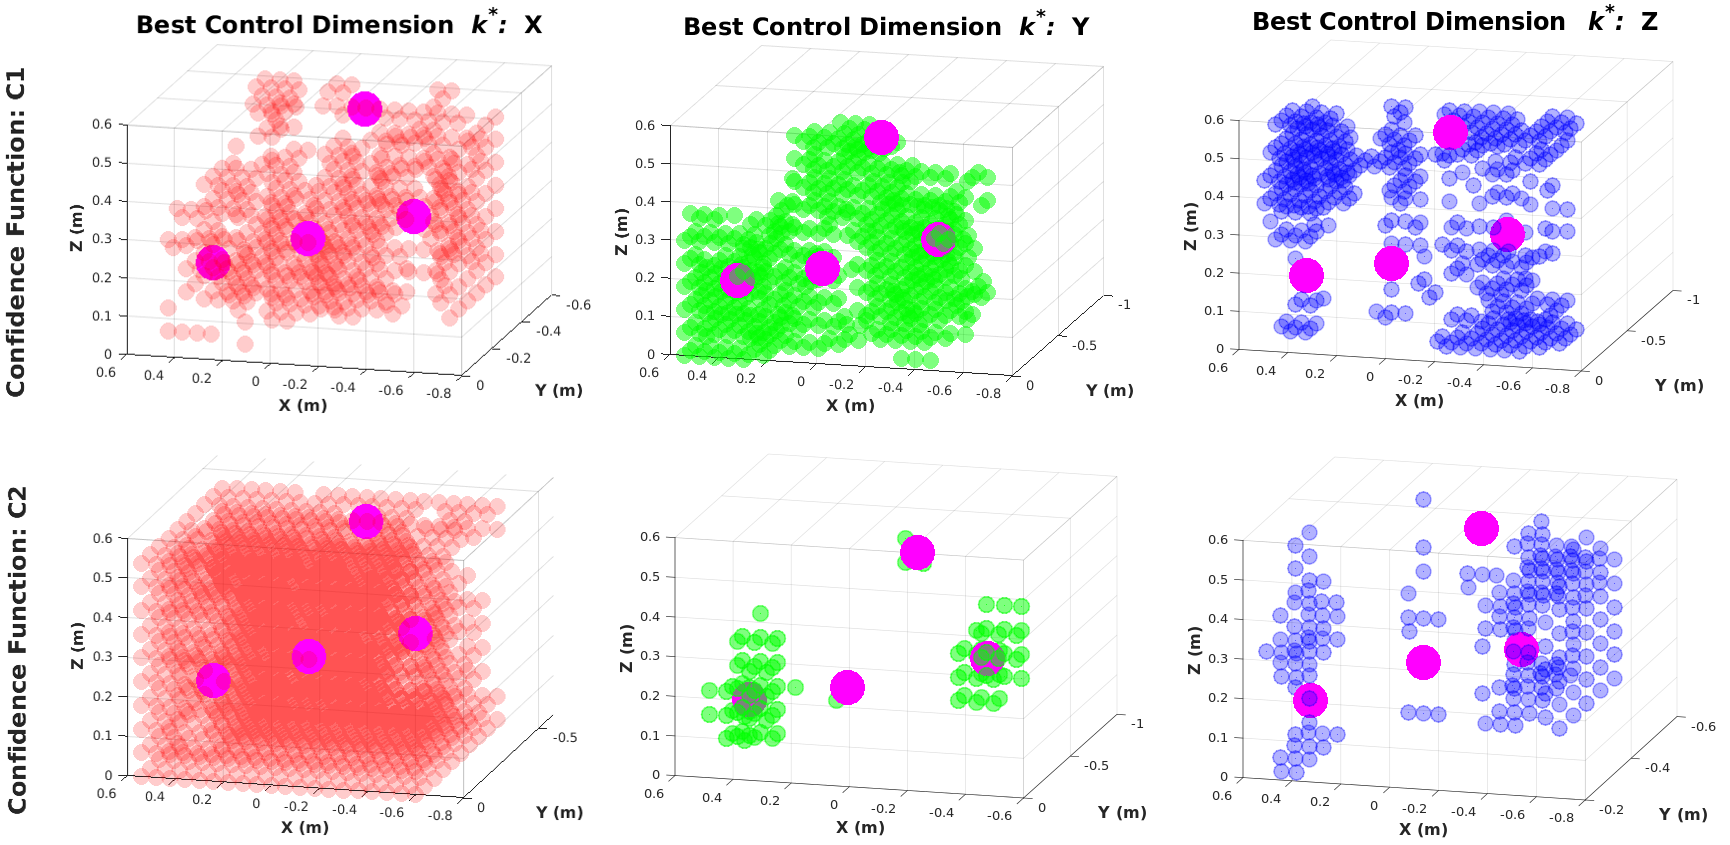
\includegraphics[width = 0.9\hsize, height = 0.35\vsize]{./figures/POINT_CLOUD.png}
	\caption{Top row: Best control dimensions for confidence measure \textbf{C1}. Bottom row: Best control dimensions for confidence measure \textbf{C2}. Left column: $\boldsymbol{k}^*$ is X. Middle Column: $\boldsymbol{k}^*$ is Y. Right Column: $\boldsymbol{k}^*$ is Z. Magenta spheres indicate the goal locations.}
	\label{HM_SEP}
\end{figure*}
The proposed disambiguation assistance paradigm augments a blending-based shared control system, in which the final control command issued to the robot is a blended sum of the human control command and an autonomous robot policy. The blending factor ($\alpha$) is a function of the system's confidence in its own estimate of the human's intent. 

Let $\boldsymbol{u}_{r,g}$ be the autonomous control policy associated with goal $g$. The final control command $\boldsymbol{u}$, issued to the robot is then given as 
\begin{equation*}
\boldsymbol{u} = \alpha\cdot \boldsymbol{u}_{r,\boldsymbol{g}^*} + (1 - \alpha)\cdot \boldsymbol{u}_h
\end{equation*}
where $\boldsymbol{g}^*$ is the most confident goal. 

The robot control command $\boldsymbol{u}_{r,g}$ is generated using a simple potential field based dynamical system which is defined in all parts of the state space. Every goal $g$ is associated with a potential field $P_g$ which treats $g$ as an attractor and all the other goals in the scene as repellers. For potential field $P_g$, the attractor velocity is given by
\begin{equation*}
\dot{\boldsymbol{x}}_{attract} = \boldsymbol{x}_{g} - \boldsymbol{x}
\end{equation*}
where $\boldsymbol{x}_{g}$ is the location of $g$. The repeller velocity is given by
\begin{equation*}
\dot{\boldsymbol{x}}_{repel} = \sum_{i \in \mathcal{G} \setminus g} \frac{\boldsymbol{x} - \boldsymbol{x}_{i}}{\eta(\norm{\boldsymbol{x} - \boldsymbol{x}_{i}}^2)}
\end{equation*}
where $\dot{\boldsymbol{x}}$ indicates the velocity of the robot in the world frame. Therefore, 
\begin{equation*}
\boldsymbol{u}_{r,g} = \dot{\boldsymbol{x}}_{attract} + \dot{\boldsymbol{x}}_{repel} 
\end{equation*}
Additionally, $P_g$ operates in full six dimensional Cartesian space and treats position and orientation as independent potential fields. 

In our implementation confidence $c_g$ is computed as
\begin{equation}\label{E1}
c_g(\boldsymbol{x}, \boldsymbol{u}_h, \boldsymbol{u}_{r,g}) = \boldsymbol{u}_{h}^{trans}\cdot(\boldsymbol{x}_{g} - \boldsymbol{x})^{trans} + \boldsymbol{u}_h^{rot}\cdot\boldsymbol{u}_{r,g}^{(rot)}
\end{equation}
where $trans$ refers to the translational and $rot$ refers to the rotational parts of the entire control space. 
\begin{figure*}[ht]
	\centering
	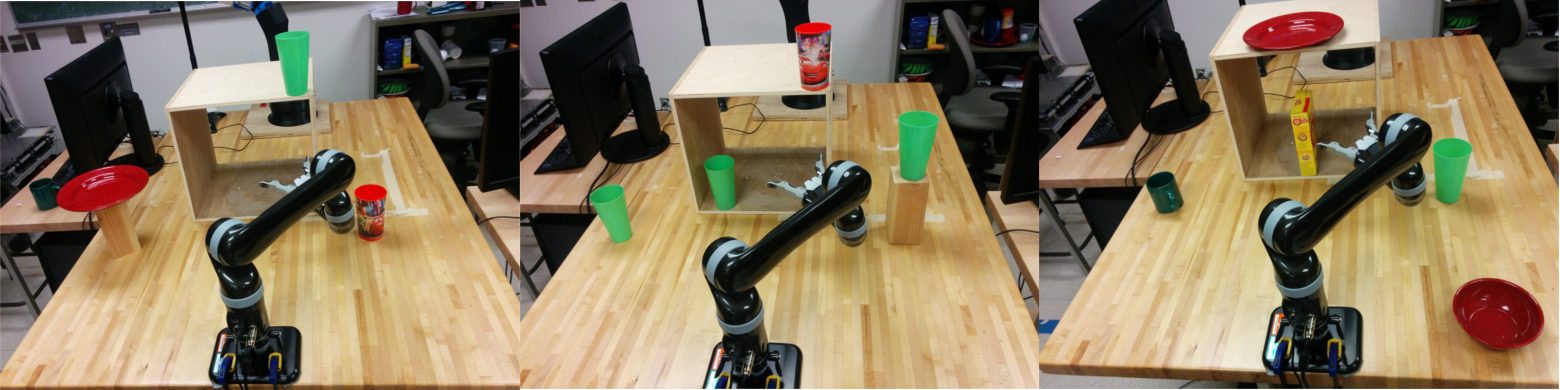
\includegraphics[width = 1\hsize]{./figures/TASKS.png}
	\caption{Pilot study tasks performed by the subjects. \textit{Left to right:} Simple Reaching (\textit{R}), Reaching with Same Grasp (\textit{RsG}), Reaching with Different Grasp (\textit{RdS}).}
	\label{TASKS}
\end{figure*}
The first term captures the ``directedness'' of the human control command towards the goal $g$ and the second term captures the alignment between the human control command and the autonomous robot policy in the rotational parts of the state space respectively. 
The blending factor $\alpha$ is a parameterized function of the confidence and is depicted in Figure~\ref{ALPHA}.
\section{EMPIRICAL VALIDATION} \label{EV}
\subsection{Robotic Platform}

The experiments were performed using real hardware and simulated versions of the MICO robotic arm (Kinova Robotics, Canada), which is a 6 DOF robotic arm specifically designed for assistive purposes. The software system was implemented using the Robot Operating System (ROS) and data analysis was performed using MATLAB. 
\subsection{Assistance Paradigms}
Three kinds of mode switching paradigms were evaluated. Note that the blending assistance was always running for all three paradigms.

\noindent\underline{\textit{Manual}}: In this paradigm the user manually performs all mode switches. The starting control mode is randomized. 

\noindent\underline{\textit{Disambiguation}}: In this paradigm, the disambiguation system is activated right at the beginning of a trial. The algorithm identifies the ``best mode'' $\boldsymbol{m}^*$ and starts the trial in control mode $\boldsymbol{m}^*$. All subsequent mode switches are performed manually by the user. Furthermore, the user is required to first move in the selected mode before manually switching the mode. 

\noindent\underline{\textit{On Demand}}: In this paradigm, the user can request a mode switch assistance at any time during task execution. This paradigm is exploratory and seeks to find underlying patterns in assistance request behavior.

\subsection{Task Descriptions}
Three tasks were developed for our pilot study (Figure~\ref{TASKS}).
\noindent\underline{\textit{Simple Reaching (R)} }: The user operates the robotic arm using both control interfaces to perform simple reaching motions to three different goal locations. This is a training task and the primary purpose is to get the user accustomed to the operation of the control interfaces, the underlying blending based assistance and the experiment protocol. 

\noindent\underline{\textit{Reaching with Same Grasp (RsG)} }: The user teleoperates the robotic arm using both control interfaces to perform reaching motions towards one of four objects on the table with the same grasp orientation.

\noindent\underline{\textit{Reaching with Different Grasp (RdG)}}: This is a more difficult task that \textit{RsG} in which the user operates the robot to perform reaching motions to one of five objects in the scene with different grasp orientations.

Analysis was performed only on data collected from \textit{RsG} and \textit{RdG}.  


\subsection{Control Interfaces}
The human control command $\boldsymbol{u}_h$ was captured using two different control interfaces: 2-axis joystick and a head array shown in Figure~\ref{J2_HA}. 
 A 2-axis joystick generates continuous signals and is capable of controlling a maximum of two control dimensions at a time. Control modes can be accessed using the buttons on the interface. 
On the other hand, head array  is a switch-based discrete teleoperation device. Head array consists of three switches; the switch at the back is used to cycle between the modes and the switches on the left and right side are to control the motion in the positive and negative direction along a control dimension. 
\begin{figure}[h]
	\centering
	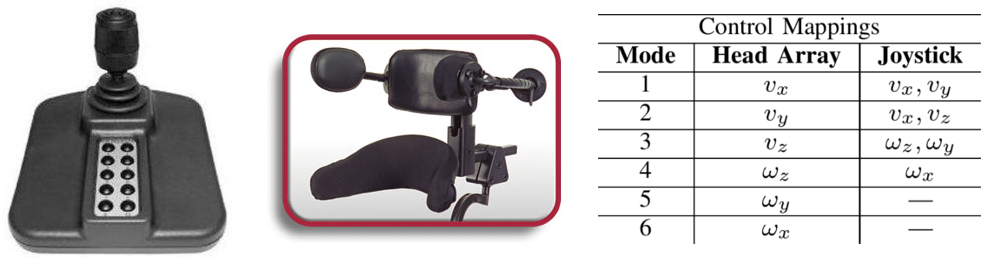
\includegraphics[width = 0.9\hsize, height = 0.16\vsize]{./figures/INTER.png}
	\caption{A 2-axis joystick (left) and switch-based head array (center) and their operational paradigms (right)}
	\label{J2_HA}
\end{figure}

%\begin{table}
%	\centering
%	\begin{tabular}{|c|c|c|}
%		\hline
%		\multicolumn{3}{|c|}{Control Mappings} \\
%		\hline
%		\textbf{Mode} & \textbf{Head Array} & \textbf{Joystick}\\
%		\hline
%		1 & $v_{x}$ & $v_{x}, v_{y}$ \\ \hline
%		2 & $v_{y}$   & $v_{x}, v_{z}$ \\ \hline
%		3 & $v_{z}$ &  $\omega_{z}, \omega_{y}$ \\ \hline
%		4 & $\omega_{z}$ &  $\omega_{x}$ \\ \hline
%		5 & $\omega_{y}$ &   --- \\ \hline
%		6 & $\omega_{x}$ &  --- \\ \hline 
%	\end{tabular}
%	\vspace{.2cm}
%	\caption{Operational paradigms for the teleoperation interfaces} 
%	\label{CIM}
%	\vspace{-.5cm}
%\end{table}

The control interface signals are mapped to Cartesian velocities of the end effector of the robot. Additionally, the interfaces can also be used to request mode switch assistance. In using two interfaces, we hope to observe an increase in task effort for the head array due to the limited bandwidth and discrete nature of the control signals. 
\section{SIMULATION RESULTS} \label{SIMRESULTS}
We first evaluate the disambiguation system for correctness within a simulated environment.

\noindent{\textbf{A}. \textit{Choice of Confidence Functions}}: Since $D_{k}$ and $D_{m}$ are evaluated using $c$ and $\frac{\partial c}{\partial k}$, they are both indirectly functions of $\boldsymbol{x}$. The choice of confidence functions can also greatly affect the computation of $\boldsymbol{k}^*$ and $\boldsymbol{m}^*$. In order to quantify the differences between different choices for confidence functions, we performed simulations in which $\boldsymbol{k}^*$ was computed at $2000$ uniformly sampled points in the workspace of the robot, approximated as a $1.2\times0.6\times0.7 m^3$ volume in front of the robot. \textbf{C1} and \textbf{C2} were chosen as the confidence functions and the goals were the same as in \textit{RsG}. 

Figure~\ref{HM_SEP} shows the results of the simulation. It is clear that the choice of confidence function changes the preferred control dimensions in the workspace quite significantly. 

More importantly, it also sheds light on the efficacy of a confidence function in capturing human intent properly. For the goal distribution used in the simulation, the goal positions are spread out maximally along the $x$ and $z$ axes. Intuitively the system will be able to quickly infer the human's intent if the human control command is either along the $x$ or the $z$ axes. However, this requires that the confidence function indeed captures the ``directedness'' of the human control command. 

Table~\ref{HMD} reports the number of times the algorithm picked each of the three control dimensions, for each confidence function.  
\textbf{C1} often was unable to capture the human intent properly. Furthermore, \textbf{C1} had ``null'' spaces where all confidences were identically equal to zero and therefore disambiguation was not possible.  
\begin{table}[t]
	\centering
	\begin{tabular}{|c|c|c|c|c|}
		\hline
		\multicolumn{5}{|c|}{Best control dimension distribution} \\
		\hline
		\textbf{Confidence Function} & \textbf{X} & \textbf{Y} & \textbf{Z} & \textbf{NULL} \\ \hline
		
		\textbf{C1} & $579$ & $615$ & $446$ & $360$ \\ \hline
		\textbf{C2} & $1711$ & $93$ & $196$ & $0$\\ \hline
		
	\end{tabular}
	\vspace{.2cm}
	\caption{Best control dimension distribution for two different confidence functions.} 
	\label{HMD}
	\vspace{-.5cm}
\end{table}

By contrast, with \textbf{C2} the algorithm identified $x$ as the preferred dimension 1711 out of 2000 samples, and $z$ in 196 of the remaining 289 samples, which indicates that the confidence function along with our algorithm was able to select the disambiguating dimensions over $95\%$ of the time. The algorithm picked $y$ only when the robot directly in front of a goal. 
\begin{table}[h]
	\centering
	\begin{tabular}{|c|c|c|c|}
		\hline
		$n_g$ & 3 & 4 & 5 \\
		\hline
		Accuracy\% & 89.24 & 87.09 & 86.11 \\
		\hline
	\end{tabular}
	\vspace{.2cm}
	\caption{Disambiguation accuracy for off-axis motions} 
	\label{SIM}
	\vspace{-.5cm}
\end{table}

\noindent{\textbf{B}. \textit{Characterization of Simplifying Assumption:}} In our algorithm, the computation of $D_{m}$ is simplified and only considers motion projected along perpendicular vectors: the axes of each dimension $k_i$ of mode $m$. However, in reality the user can generate a control command in any arbitrary direction within the control mode, and so the robot can move along any vector spanned by the control dimensions in $m$. In order to assess whether the simplification was indeed sufficient to characterize the disambiguation capability of being in a mode, we performed simulations in which $\boldsymbol{m}^*$ was computed for $500$ uniformly spaced locations in the robot workspace. At each of those points, $100$ random control commands that are feasible in $\boldsymbol{m}^*$ were generated and applied to perturb the robot. Finally, at each of these perturbed positions the best control mode was once again computed. 

If the best mode in the perturbed position was the same mode as $\boldsymbol{m}^*$, then the simplification did not adversely affect the identification of the disambiguating mode. Table~\ref{SIM} summarizes the number of times a match occurred for different configurations of the workspace (number of goals). While the simplification holds for $85-90\%$ of off-axis motions, we do observe a trend where performance drops as the number of goals increase. Intuitively this makes sense because disambiguation between goals will become harder as the number of goals increase. 
 
\noindent{\textbf{C}. \textit{Discussion (part 1)}}:  Our simulation results indicate that the choice of confidence function has a huge impact on the performance of our algorithm. Confidence functions that encode the ``directedness'' present in the human control command are likely to be more effective in capturing human intent.
 Moreover, the algorithm can be used to pre-compute the best modes ahead of time and can be used as a look-up table during task execution for automated mode switching. A single mode switch assistance provided at the beginning of the trial might not be enough to and therefore automated mode switching during task execution will be critical to improve task performance especially for more limited interfaces. 
\section{PILOT STUDY}\label{EXP}
We next investigate the use and utility of our disambiguation approach in a pilot study. Four subjects participated in the pilot study, (3 male, 1 female), and all were lab members.


\subsection{Pilot Study Protocol and Metrics}

\noindent\underline{\textit{Protocol}}:
A within-subject study was conducted using a full factorial design in which the manipulated variables are the tasks, control interfaces and assistance paradigms. Each task consisted of two phases. 

In phase I, each user performed the task using both interfaces under \textit{Manual} and \textit{Disambiguation} paradigms. The trials were balanced and the control interfaces and the paradigms were randomized to eliminate ordering effects. The starting positions of the robot were also randomized to avoid biases. Three trials were collected for each permutation of manipulated variables. 
In phase II, the user performed the same task using both interfaces using the \textit{on-demand} paradigm and two trials were collected for each task-interface combination.  

\noindent\underline{\textit{Metrics}}: A number of objective metrics were evaluated during this pilot study. \textit{Task completion time} is the amount of time a user spends in accomplishing a task. \textit{Mode switches} refer to the number of times the user switched between various modes while performing the task and is an indicator of effort. 
%Subjective evaluation was also performed at the end of the trials for each task--interface combination in which the user was required to answer a short survey containing questions regarding the utility value,  user acceptance and the synergy in human-robot interaction as perceived by the user.  

%\section{RESULTS} \label{RES}
%\subsection{Simulation Results}

\subsection{Pilot Study Results}\label{RES}
An improvement in task performance in terms of a decrease in the number of mode switches was observed across all task--interface combinations. Statistical significance in Figure~\ref{DATAPLOT} is determined by two-sided Wilcoxon Rank-Sum Test, where (*) indicates $p < 0.05$.

	\begin{figure}[t]
	\centering
	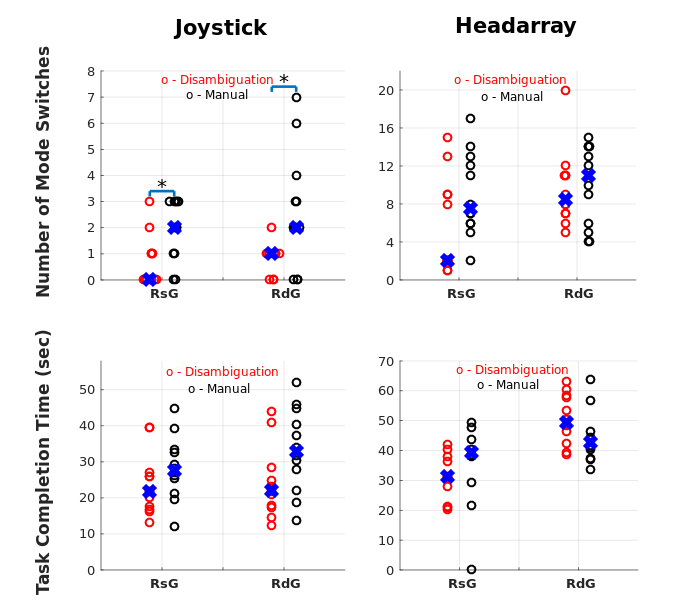
\includegraphics[width = 1.07\hsize,center]{./figures/DATA_PLOT.png}
	\vspace{-0.7cm}
	\caption{Comparison of Disambiguation and Manual paradigms. Operation using a joystick (left column) and head array (right column) interfaces. Evaluation of mode switches (top row) and completion time (bottom row).}
	\label{DATAPLOT}
\end{figure}
\vspace{0.1cm}
\noindent{\underline{\textit{Mode Switches}}}: Figure~\ref{DATAPLOT} (top row) reveals the general trend of a decrease in the number of mode switches across all task-interface combinations. However, the difference in the number of mode switches was statistically significant only when using the joystick. This indicates that upon starting in a mode identified by the algorithm, the number of subsequent mode switches performed by the user was reduced. 

\vspace{0.1cm}
\noindent{\underline{\textit{Task Completion Time}}}: In Figure~\ref{DATAPLOT} (bottom row), a decrease in task completion times during \textit{Disambiguation} paradigm was observed in all but one case: \textit{RdG}--headarray combination. However, these differences were not statistically significant for any of the task-interface combinations. The anomalous case of an increase in task completion time for \textit{RdG}--headarray combination can be explained by the fact that a \textit{single} mode switch assistance at the beginning of the trial probably did not have measurable impact as the task required multiple mode switches to operate in the orientation space as well.

\vspace{0.1cm}
\noindent{\underline{\textit{On--Demand}}}: The number of disambiguation requests for each task-interface combinations is reported in Table~\ref{ONDEMAND}. Although the subjects demonstrated a wide range of disambiguation request behaviors, we were able to observe a general trend of an increase in disambiguation requests with an increase in task difficulty. This shows that users were keen to explore the \textit{on-demand} option when the tasks became more difficult. 

%\noindent{\underline{\textit{Subjective Data}}}: Users rated the utility value of the mode switch assistance system fairly high (mean = $4.31\pm0.87$) across all task--interface combination. The user acceptance was also fairly good (mean = $4.75\pm1.183$). The users also felt that there was good synergy between the robot and themselves during task execution (mean = $5.8 \pm 0.40$). Three out of the four subjects preferred \textit{on demand} paradigm the most and the fourth subject preferred \textit{manual}. Head array was rated as the harder interface to operate the robot among the two. 
%\begin{table}
%	\centering
%	\begin{tabular}{|l|c|c|c|c|}
%		\hline
%		\multicolumn{5}{|c|}{Best control dimension distribution} \\
%		\hline
%		\textbf{Confidence Function} & \textbf{X} & \textbf{Y} & \textbf{Z} & \textbf{NULL} \\ \hline
%		
%		$\max(0, 1-d/D)$ & $579$ & $615$ & $446$ & $360$ \\ \hline
%		$\boldsymbol{u}_h\cdot(\boldsymbol{x}_{g^i} - \boldsymbol{x})$ & $1711$ & $93$ & $196$ & $0$\\ \hline
%	\end{tabular}
%	\vspace{.2cm}
%	\caption{Operational paradigms for the teleoperation interfaces} 
%	\label{ONDEMAND}
%	\vspace{-.5cm}
%\end{table}


\begin{table}
	\centering
 \begin{tabular}{ccccc}
	\toprule
	&\multicolumn{2}{c}{Joystick}
	&
	\multicolumn{2}{c}{Head Array} \\\cmidrule(r){2-3}\cmidrule(l){4-5}
	SubID &\textit{RsG}& \textit{RdG}    & \textit{RsG} &\textit{RdG}      \\
	\bottomrule
	H1 &1& 0   & 5 & 6  \\
	\bottomrule
	H2 &1& 1    & 3 & 6      \\
	\bottomrule
	H3 &2& 2    & 4 &5    \\
	\bottomrule
	H4 &2& 5    & 17 &7   \\
	\bottomrule
\end{tabular}
\vspace{.2cm}
\caption{Number of Disambiguation requests}
\label{ONDEMAND}
\end{table}

\subsection{Discussion}
Currently the algorithm assumes that at any point in the workspace all the goals in the scene are equally likely. However, in the real scenario, the user usually has an idea of what goal s/he is going for. Therefore, it might be useful to bias the computation of the ``best control mode'' by looking for cues in the past history of the robot trajectory and control commands such that the control mode chosen will always be useful for the human in reaching the goal s/he has in mind. This will also likely improve the robustness and result in higher user acceptance. 
Secondly, the algorithm only tries to maximize the utility value \textit{for} the robot. Concepts from decision theory can be used to augment the current framework to also include a utility function \textit{for} the human. A more extensive user study with motor-impaired subjects will be conducted in the future to evaluate the utility value of the disambiguation assistance system and further explore and understand the disambiguation request patterns of users. 
%\begin{table}
%	\centering
%	\begin{tabular}{ccccc}
%		\toprule
%		&\multicolumn{2}{c}{Joystick}
%		&
%		\multicolumn{2}{c}{HeadArray} \\\cmidrule(r){2-3}\cmidrule(l){4-5}
%		Questions &T1& T2    & T1 &T2      \\
%		\bottomrule
%		Utility &4.50 $\pm$ 1.00& 4.75 $\pm$ 0.50  & 4.25 $\pm$ 1.26 & 3.75 $\pm$ 0.50  \\
%		\bottomrule
%		Acceptance &4.75 $\pm$ 1.50& 5.00 $\pm$ 0.81  & 5.00 $\pm$ 1.41 & 4.25 $\pm$ 1.26      \\
%		\bottomrule
%		Synergy &5.75 $\pm$ 0.50&  6.00 $\pm$ 0.00   & 5.75 $\pm$ 0.50 &5.75 $\pm$ 0.5   \\
%		\bottomrule
%	\end{tabular}
%	\vspace{.2cm}
%	\caption{User responses on perceived utility, acceptance and synergy}
%	\label{US}
%\end{table}
\section{CONCLUSIONS}\label{DC}

In this paper, we have presented an algorithm for disambiguation assistance with a shared-control robotic arm. We also introduced the notion of \textit{inverse legibility}, in which the human-generated actions are legible enough \textit{for} the robot to infer the human intent confidently and accurately. The goal of the algorithm developed in this paper is to seek legible control commands from the human by placing the control in those modes able to \textit{maximally disambiguate} between the various goals in the scene.  Moreover, preliminary pilot study results indicated that the disambiguation paradigm proposed was successful in decreasing task effort (number of mode switches) across interfaces and tasks. Our simulation work evaluated the robustness of the algorithm and the impact of different confidence functions on intent disambiguation. In our future work, informed by our pilot studies we plan to enhance our algorithm, to improve task performance and extend the framework into an automated mode switch assistance system. 

\section*{Acknowledgments}
Funding source omitted for review. 
%\subsection{Subsection Heading Here}
%Subsection text here.
%
%\subsubsection{Subsubsection Heading Here}

%
%
%\section{RSS citations}
%
%Please make sure to include \verb!natbib.sty! and to use the
%\verb!plainnat.bst! bibliography style. \verb!natbib! provides additional
%citation commands, most usefully \verb!\citet!. For example, rather than the
%awkward construction 
%
%{\small
%\begin{verbatim}
%\cite{kalman1960new} demonstrated...
%\end{verbatim}
%}
%
%\noindent
%rendered as ``\cite{kalman1960new} demonstrated...,''
%or the
%inconvenient 
%
%{\small
%\begin{verbatim}
%Kalman \cite{kalman1960new} 
%demonstrated...
%\end{verbatim}
%}
%
%\noindent
%rendered as 
%``Kalman \cite{kalman1960new} demonstrated...'', 
%one can
%write 
%
%{\small
%\begin{verbatim}
%\citet{kalman1960new} demonstrated... 
%\end{verbatim}
%}
%\noindent
%which renders as ``\citet{kalman1960new} demonstrated...'' and is 
%both easy to write and much easier to read.
%  
%\subsection{RSS Hyperlinks}
%
%This year, we would like to use the ability of PDF viewers to interpret
%hyperlinks, specifically to allow each reference in the bibliography to be a
%link to an online version of the reference. 
%As an example, if you were to cite ``Passive Dynamic Walking''
%\cite{McGeer01041990}, the entry in the bibtex would read:
%
%{\small
%\begin{verbatim}
%@article{McGeer01041990,
%  author = {McGeer, Tad}, 
%  title = {\href{http://ijr.sagepub.com/content/9/2/62.abstract}{Passive Dynamic Walking}}, 
%  volume = {9}, 
%  number = {2}, 
%  pages = {62-82}, 
%  year = {1990}, 
%  doi = {10.1177/027836499000900206}, 
%  URL = {http://ijr.sagepub.com/content/9/2/62.abstract}, 
%  eprint = {http://ijr.sagepub.com/content/9/2/62.full.pdf+html}, 
%  journal = {The International Journal of Robotics Research}
%}
%\end{verbatim}
%}
%\noindent
%and the entry in the compiled PDF would look like:
%
%\def\tmplabel#1{[#1]}
%
%\begin{enumerate}
%\item[\tmplabel{1}] Tad McGeer. \href{http://ijr.sagepub.com/content/9/2/62.abstract}{Passive Dynamic
%Walking}. {\em The International Journal of Robotics Research}, 9(2):62--82,
%1990.
%\end{enumerate}
%%
%where the title of the article is a link that takes you to the article on IJRR's website. 
%
%
%Linking cited articles will not always be possible, especially for
%older articles. There are also often several versions of papers
%online: authors are free to decide what to use as the link destination
%yet we strongly encourage to link to archival or publisher sites
%(such as IEEE Xplore or Sage Journals).  We encourage all authors to use this feature to
%the extent possible.
%
%\section{Conclusion} 
%\label{sec:conclusion}
%
%The conclusion goes here.

%\section*{Acknowledgments}

%% Use plainnat to work nicely with natbib. 

\bibliographystyle{plainnat}
\bibliography{references}

\end{document}


